% Template made by Mohsen Toorani
% Last update 2024-06-05
\documentclass[a4paper, 10pt]{article}
\usepackage[utf8]{inputenc}
\usepackage[includeheadfoot,margin=0.9in]{geometry}
\usepackage[T1]{fontenc}
\usepackage{times}
\usepackage[english]{babel} % bytt ut engelsk med norsk dersom du ønsker det
\usepackage{graphicx}
\usepackage[export]{adjustbox}
\usepackage{hyperref}
\usepackage{footnote}
\usepackage{float}
\usepackage{enumitem}
\makesavenoteenv{tabular}
\makesavenoteenv{table}
\usepackage{nopageno}
\usepackage[colorinlistoftodos]{todonotes}
\pagenumbering{arabic}
\usepackage[none]{hyphenat}
\usepackage{fancyhdr}
\pagestyle{fancy}
\fancyhf{}

\setlength{\headheight}{32.09pt}
\fancyhead[L]{
\includegraphics[height=1cm]{USN.png}}
\fancyhead[R]{Data Mining and Business Analytics}
\cfoot{\thepage}
\rfoot{Student name: Frodo Baggins} % replace XX with your name. 

% Defining \maketitle
\makeatletter
\def\@maketitle{
\raggedright

\includegraphics[width = 125mm]{USNlogo.png}\\[10ex]
\begin{center}
{\Huge \bfseries \sffamily \@title}~\\[4ex] 
{\Large  \@author}~\\[4ex] 
\@date
\end{center}}
\makeatother

\newcommand*\wildcard[2][5cm]{\vspace*{2cm}\parbox{#1}{\hrulefill\par#2}}

\title{One Thesis to Rule Them All: An Academic Journey by Frodo Baggins, Guided by Bilbo and Gandalf  \\ [3ex] % replace this line with your own title

%\large Project Proposal for Master's Thesis \\[2ex]
}  % This line should remain as it is

% Replace XX in following lines with your information
\author{
  Student name: Frodo Baggins \\ [2ex]
  Student number: 001 \\ [2ex] 
  Email address: \texttt{fbaggins@usn.no} \\ [2ex]
  Academic supervisor: Bilbo Baggins \\ [1ex]
  Co-supervisor (Industry): Gandalf\\ [10ex]
}



\begin{document}

\maketitle
\thispagestyle{empty}
\newpage

\begin{abstract}
Skriv en kort oppsummering av oppgaven her (maks 250 ord)
\end{abstract}

\section{Introduction/Introduksjon}

Introduksjonsdelen av oppgaven skal inneholde nødvendig bakgrunnsinformasjon, inkludert en tilstrekkelig gjennomgang av tidligere funn og begrunnelsen for å gjennomføre denne studied. Husk å sitere~\cite{attention_is_all_you_need}

\section{Method/Metode}
I metode-avsnittet, vennligst beskriv alle nødvendige
detaljer om hvordan studien ble utført. Informasjon bør være grundig og objektiv slik at andre kan reprodusere arbeidet ditt.
Egne meninger og tolkninger hører ikke hjemme her. Spar disse til diskusjons-delen.

Formler kan du skrive på denne måten: \begin{equation}
\int_0^\infty e^{-x^2}dx = \frac{\sqrt{\pi}}{2}.
\label{eq:label}
\end{equation}

Eller innfelt i teksten på denne måten $y = x^2$

\section{Results/Resultater}
Bruk denne delen til å presentere resultatene fra arbeidet du har utført. Unngå diskusjon av resultatene, den kommer i neste kapittel.

Figurer og tabeller kommer vanligvis i dette avsnittet. Husk å referere til bildene og tabellene i teksten. Figur~\ref{fig:label1} viser ...
og av Tabell~\ref{fig:label1} ser vi at ...

\begin{figure}[h]
\centering
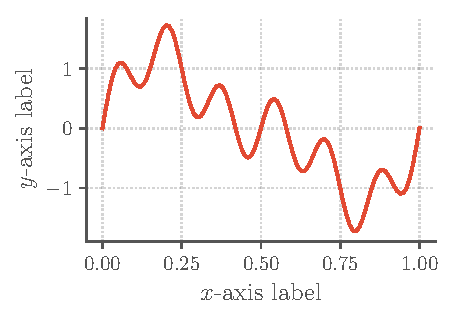
\includegraphics{example_figure}
\caption{Skriv en figurtekst som forklarer figuren din}
\label{fig:label1}
\end{figure}

\begin{table}[h]
\centering
\caption{Dette er tabellteksten}
\begin{tabular}{c|c}
    \hline
    Column A & Column B \\\hline
    1.2      & 3.4      \\
    5.6      & 7.8      \\\hline
\end{tabular}

\label{tab:label}
\end{table}

\section{Discussion/Diskusjon}
Nå kan du diskutere resultatene dine. Legg vekt på de nye og viktige
aspektene ved studien du har utført.

\section{Conclusion/Konklusjon}
Skriv en kort oppsummering av hva du har gjort, hva du fant og implikasjonene av funnene dine i det store bildet.

\bibliographystyle{ieeetr}
\bibliography{ref}

% Replace XX in the below fields with names of corresponding persons.


\end{document}